\documentclass{article}
\usepackage{amsmath}
\usepackage{amssymb}
\usepackage{graphicx}
\usepackage{hyperref}
\usepackage[version=4]{mhchem}


\begin{document}
\section*{Problem}
\(A B C D\) is a convex quadrilateral. \(M\) and \(N\) are midpoints of \(A D, B C\), respectively. Show that \(M N \leq \frac{1}{2}(A B+D C)\).\\
\centering
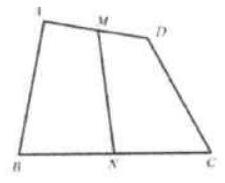
\includegraphics[width=\textwidth]{images/044(4).jpg}

\section*{Solution}
If \(A B / / D C, A B C D\) is a trapezoid \(A B C D\).\\
By Theorem 2.3, \(M N=\frac{1}{2}(A B+D C)\).\\
Otherwise, Connect \(A C\). Take \(P\), the midpoint of \(A C\). Connect \(P A, P N\).\\
Since \(M\) and \(P\) are midpoints of \(A D, A C\), respectively, by Theorem 2.1,\\
\(M P=\frac{1}{2} D C\)\\
Since \(N\) and \(P\) are midpoints of \(B C, A C\), respectively, by Theorem 2.1,\\
\(N P=\frac{1}{2} A B\)\\
(1) \(+(2): M P+N P=\frac{1}{2}(D C+A B)\)

By the triangle inequality theorem, \(M P+N P>M N\).\\
\centering
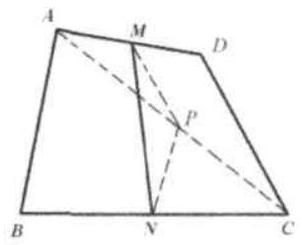
\includegraphics[width=\textwidth]{images/049.jpg}

Thus \(M N<\frac{1}{2}(A B+D C)\).


Therefore, we have \(M N \leq \frac{1}{2}(A B+D C)\).

\end{document}
